\documentclass[12pt]{article}

\usepackage{graphicx}

\title{Evolutionary Mechanics}
\author{Tobias Jacob, Raffaele Guillera, Ali Muddasar}

\begin{document}
    \maketitle
    \begin{abstract}
        We developed an application that is able to develop mechanical structures using an evolutionary algorithm. This approach can be scaled efficiently across many different nodes.
    \end{abstract}
    \section{Method}
    Our project is divided in two sections and corresponding layers of parallelism. The first one is solving the mechanical equations to check if a mechanical structure can withstand a force.
    \begin{figure}[t]
        \centering
        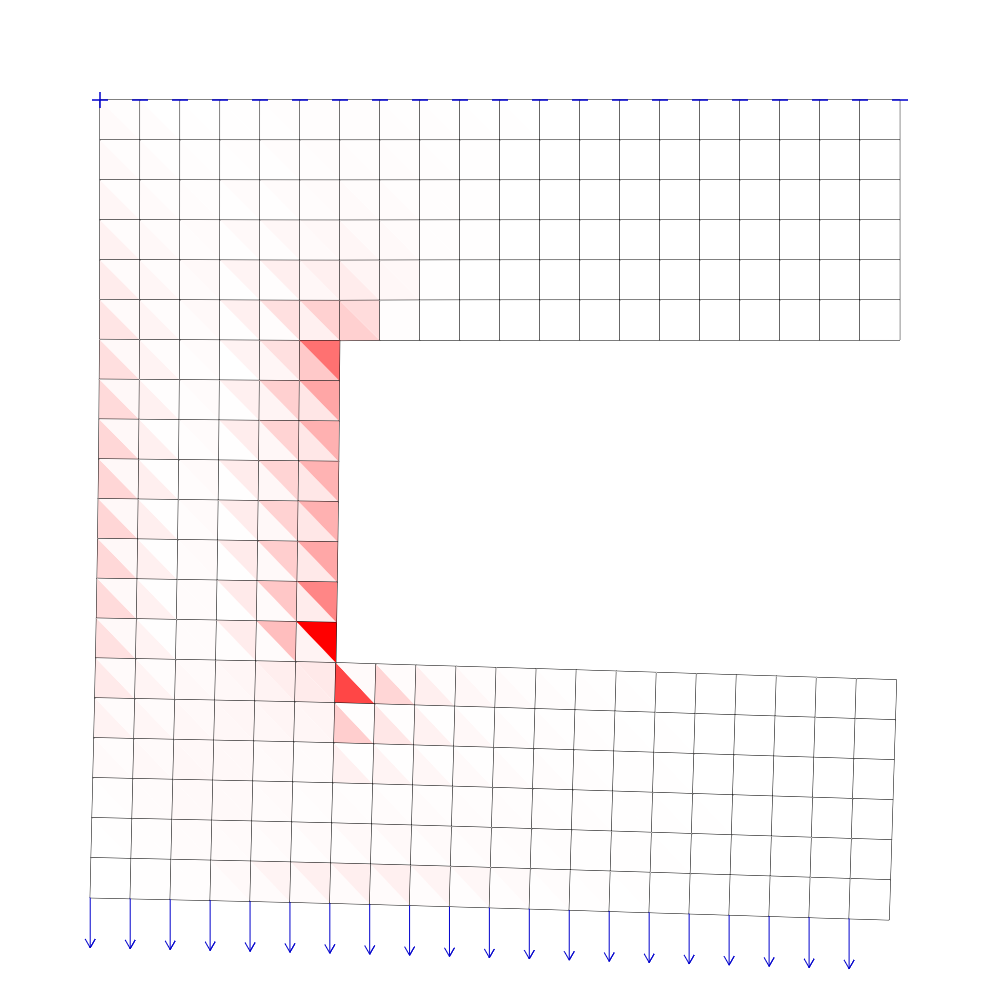
\includegraphics[width=0.8\textwidth]{images/MechaincalStructure.png}
        \caption{Result of a mechanical simulation}
        \label{fig:Mechanical_Simulation}
    \end{figure}
    Figure~\ref{fig:Mechanical_Simulation} 
\end{document}